%%This is a very basic article template.
%%There is just one section and two subsections.
\documentclass{article}

\usepackage{hyperref}
\usepackage{graphicx,subfigure,wrapfig}

\begin{document}

\title{Statechart ProM Plugin -- User Manual\\ \vspace*{0.6em} 
{\large Statechart Workbench: Process Exploration Workflow Tool\\ \vspace*{-0.4em} 
Supporting Hierarchy, Recursions, Cancellations and Software Logs
}}
\author{M.~Leemans (\href{mailto:m.leemans@tue.nl}{m.leemans@tue.nl})}
\maketitle

\section{Introduction}
The Statechart Workbench can be used to discover models with \emph{hierarchy},
\emph{recursion} and \emph{cancellation} from ordinary event logs.
The models can be displayed as \emph{statecharts}, \emph{sequence diagrams}, \emph{Petri nets} and other visual formalisms.
The Statechart Workbench is a process exploration workflow tool and it provides 
an easy and guided approach to apply a collection of advanced algorithms. 

The original purpose of the Statechart Workbench was to analyse event logs
obtained from instrumented software, but the tool is able to handle any 
ordinary (business) event log.
To start analysing your own software, create a software event log using
the instrumentation tool available at: \url{https://svn.win.tue.nl/repos/prom/XPort/}.

\section{Installation}
There are two ways to install and use the Statechart Workbench.
The default way is to install the \emph{Statechart} plugin via the ProM Package Manager.
Recent nightly builds should already have this plugin installed by default.
The ProM nightly build can be found at: \url{http://www.promtools.org/doku.php?id=nightly}.

Alternatively, one can checkout the source code repository, 
and load the Eclipse launch file \emph{ProM with UITopia (Statechart-hg).launch}.
Note: you can import this codebase as an existing Eclipse project.

\section{Getting Started}
In this section, step-by-step instructions are given to get started with the Statechart Workbench.
For this guide we use JUnit software event log, publicly available at: 
\url{https://doi.org/10.4121/uuid:cfed8007-91c8-4b12-98d8-f233e5cd25bb}.

\subsection{Step 1: Load an event log}
To get started, first load an event log into ProM as usual.
You can either drag an XES log onto ProM, or use the \emph{Import} button on 
the top right.

Next, launch the Statechart Workbench.
The preferred way to do this is to simply launch the \emph{Statechart Workbench} log visualizer:
\begin{enumerate}
  \item View the event log resource (Figure~\ref{fig:start:view}).
  \item Launch the \emph{Statechart Workbench} log visualizer (Figure~\ref{fig:start:vis}).
\end{enumerate}
Alternatively, one can start the \emph{Discover using the Statechart Workbench} plugin action (Figure~\ref{fig:start:plugin}).

\begin{figure}[hb!]
\centering
\vspace*{-0.5em}
    \subfigure[Step 1 -- Viewing an event log]{
      \label{fig:start:view}
      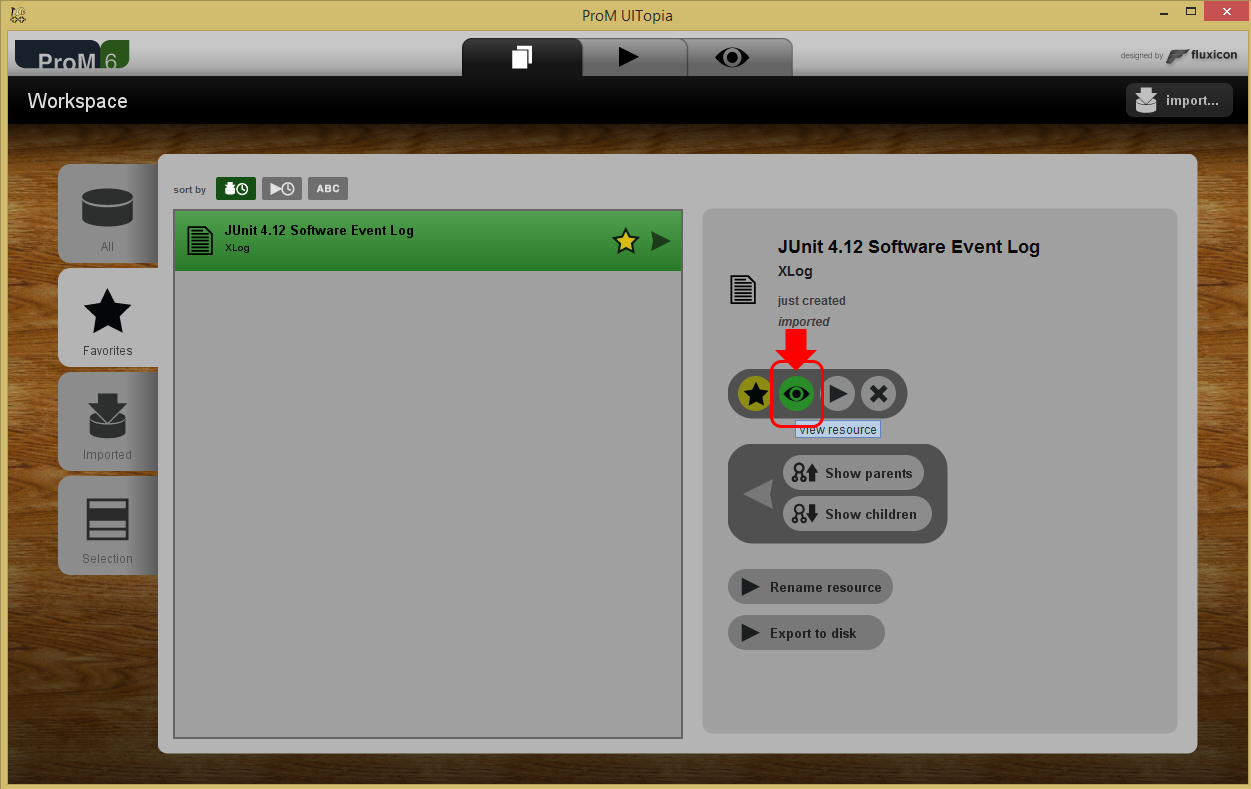
\includegraphics[width=0.8\textwidth]{gfx/start-view.png}
    }
\vspace*{-1em}
    \subfigure[Step 2 -- Launching the \emph{Statechart Workbench} log visualizer.]{
      \label{fig:start:vis}
      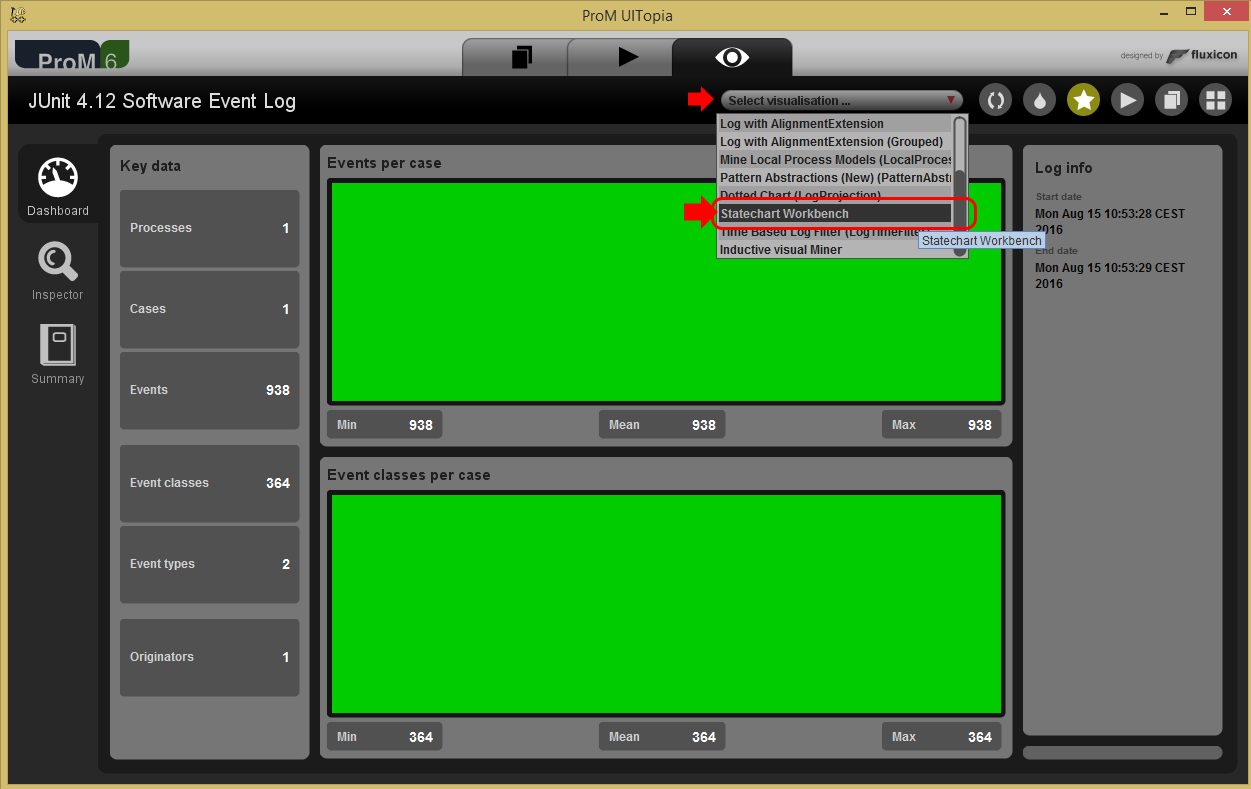
\includegraphics[width=0.8\textwidth]{gfx/start-vis.png}
    }
\caption{Lauching the \emph{Statechart Workbench} log visualizer.}
\label{fig:start}
\vspace*{-0.5em}
\end{figure}

\begin{figure}[ht!]
\centering
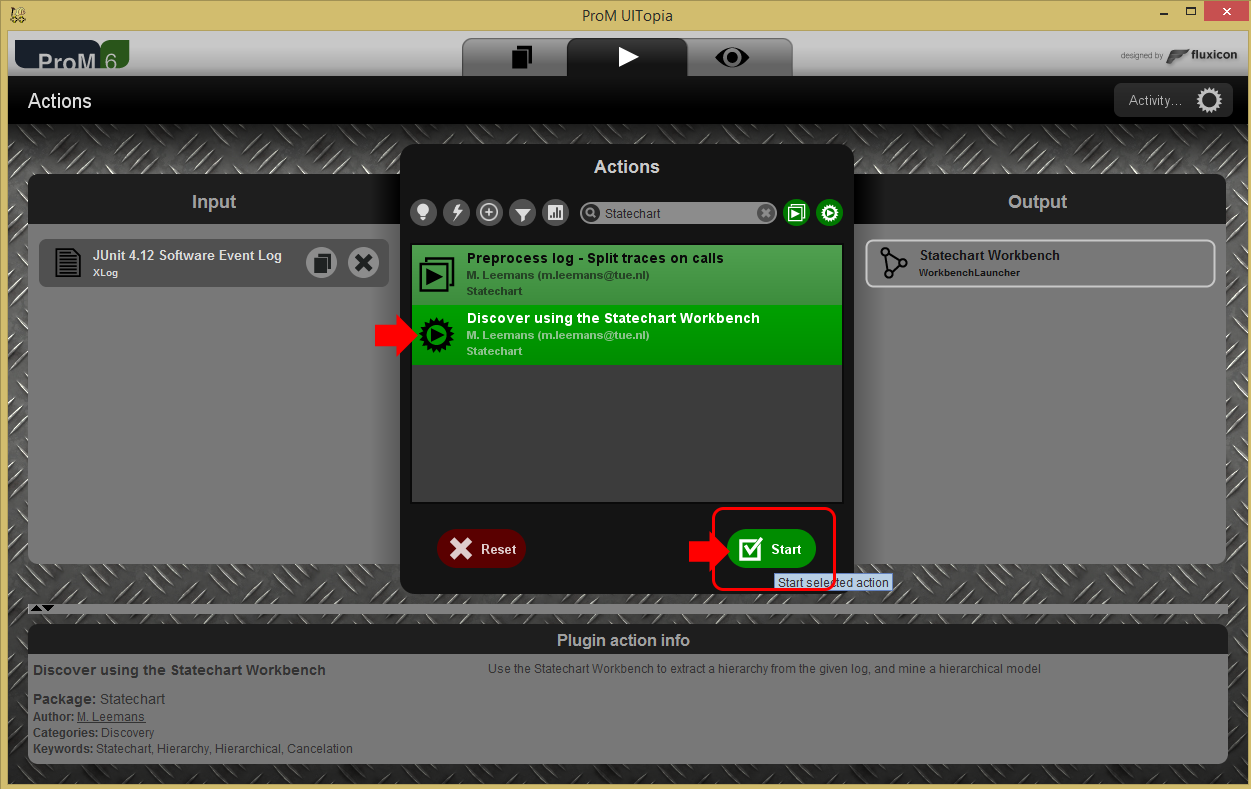
\includegraphics[width=0.8\textwidth]{gfx/start-plugin.png}
\caption{Launching the \emph{Discover using the Statechart Workbench} plugin action.}
\label{fig:start:plugin}
\end{figure}

\subsection{Step 2: Setup Key Heuristics}
The Statechart Workbench implements a simple workflow.
First, you setup some key heuristics: \emph{Hierarchy} and \emph{Cancelation}.
After that, the discovered model is shown in the the \emph{Discovery \& Analysis screen} screen,
allowing you to explore and and perform analyses.
In the top left corner of the Statechart Workbench (see Figure~\ref{fig:setup}), 
the workflow and the current step is shown in three big chevrons.

Hierarchy and Cancelation are two key heuristics in the Statechart Workbench that require some setup.
Before you can start discovering a model, you need to select a strategy for these heuristics.
In most cases, you can choose one of the two quick presets, see also Figure~\ref{fig:setup}:
\begin{itemize}
  \item \textbf{Start Discovery -- Normal Log} This preset covers most normal logs: no special hierarchy or cancelation is setup.
  \item \textbf{Start Discovery -- Software Log} This preset covers most software logs: the default software hierarchy and cancelation heuristics are used.
\end{itemize}

For the JUnit example log, we can just select the \textbf{Start Discovery -- Software Log} preset.
If you choose a preset, you immediately jump to the \emph{Discovery \& Analysis screen} screen, see Section~\ref{sec:discovery}.
If you choose to configure the heuristics manually, you get to option to select a hierarchy heuristic, and afterwards a cancellation heuristic.

\phantom\newline
\textbf{Note: Classifier Selection}
The acitvity classifier used for discovery is set in the hierarchy heurstic.

\begin{figure}[ht!]
\centering
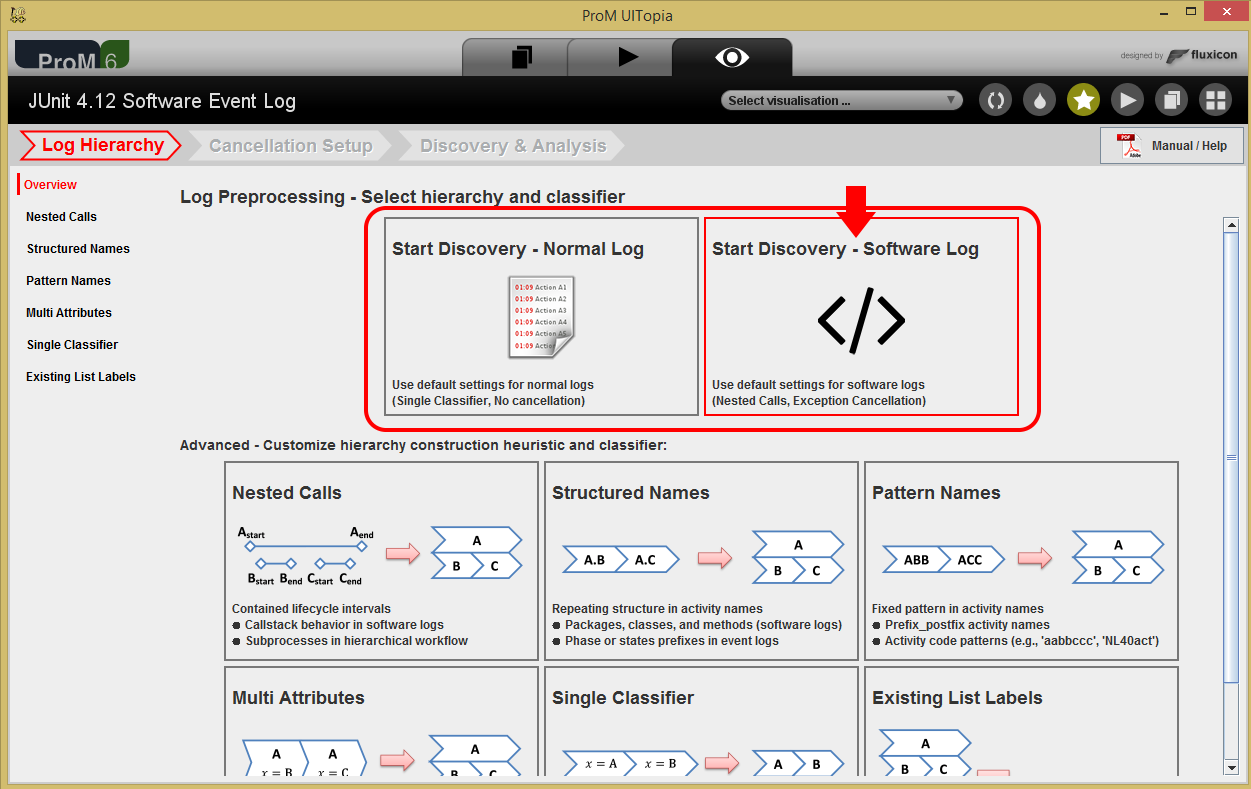
\includegraphics[width=0.8\textwidth]{gfx/setup.png}
\caption{Initial screen when launching the \emph{Statechart Workbench}: the setup of the key heuristics. In red are the two quick preset options.}
\label{fig:setup}
\end{figure}

\subsubsection{Log Hierarchy}
There are several heuristics options for creating a log hierarchy.
In short, a hierarchy heuristics tries to create a multi-level (hierarchical) structure over the event log,
such that the discovery algorithm can discover hierarchy, subprocesses and recursions.
The available heuristics options are shown on the home screen in blocks, and listed on the sidebar to the left, see also Figure~\ref{fig:setup}.
Each heuristics option is explained in the tool with a visual cue and a description. 

\subsubsection{Cancellation Setup}
After setting up a hierarchy, there are several heuristics options for creating a cancellation oracle.
In short, a cancelation oracle tries to creater a reference map of activities that
are potentially involved in cancellation patterns.
The cancelation oracle aides the discovery algorithm in finding these cancellation regions.
The available heuristics options are shown on the \emph{Cancellation Setup} screen in blocks, and listed on the sidebar to the left.
Each heuristics option is explained in the tool with a visual cue and a description. 

\subsection{Step 3: Discovery and Analysis}
\label{sec:discovery}
After choosing a preset or setting up the heuristics, you end up on the \emph{Discovery \& Analysis screen}, see Figure~\ref{fig:discovery}.
In the center of this screen, the discovered model is shown.
On the left, a list of all the activities is shown.
And on the right, the options and settings are shown.
Using the three big chefrons at the top, different hierarchy can cancellation heuristics can be set.

\begin{figure}[h!]
\centering
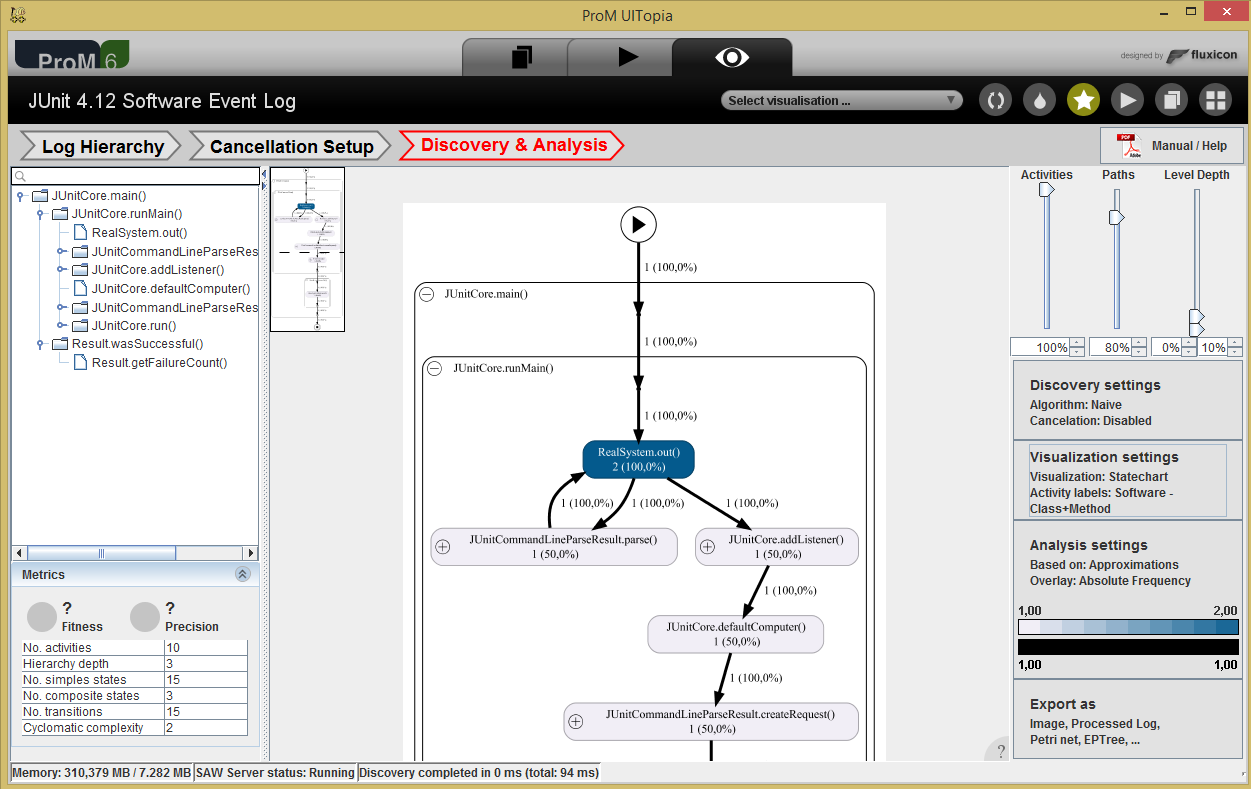
\includegraphics[width=0.8\textwidth]{gfx/discovery.png}
\caption{Discovery \& Analysis screen screen of the Statechart Workbench.}
\label{fig:discovery}
\end{figure}

\subsubsection{Center panel: Discovered Model}
The center panel shows the discovered model.
By dragging the screen (left-click and hold on the model), you can move through the model.
By using the scroll wheel, you can zoom in and out.
By left clicking on a node, you can open up a detailed popup with more information (Figure~\ref{fig:screen:popup}).

In the case of hierarchical models, the plus and minus signs allow you to expand and collapse a subprocess / hierarchy level.

\paragraph{Source Code Link}
If you're using the SAW Eclipse plugin available via
\url{https://svn.win.tue.nl/repos/prom/XPort/},
you can link the shown software model back to the source code.
When a model is discovered, you can connect to the SAW server in the current Statechart Workbench,
see Figure~\ref{fig:connect}.
The status of the SAW server is shown at the bottom of the screen.
Once connected, a double click on a model node will trigger the SAW Eclipse plugin
to open the corresponding source code line.

\begin{figure}[h!]%
    \centering%
    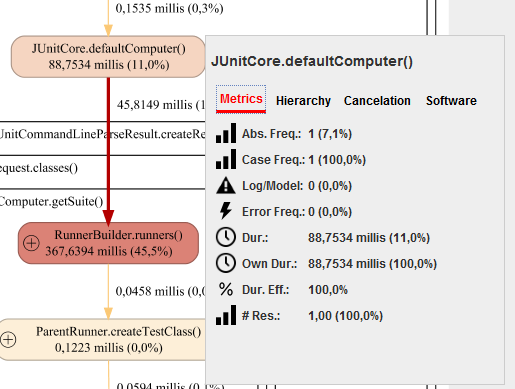
\includegraphics[width=0.8\textwidth]{gfx/model-popup.png}%
    \caption{Clicking on a model element opens up an info popup with several tabs of detailed information.}%
    \label{fig:screen:popup}%
\end{figure}%

\begin{figure}[h!]
\centering
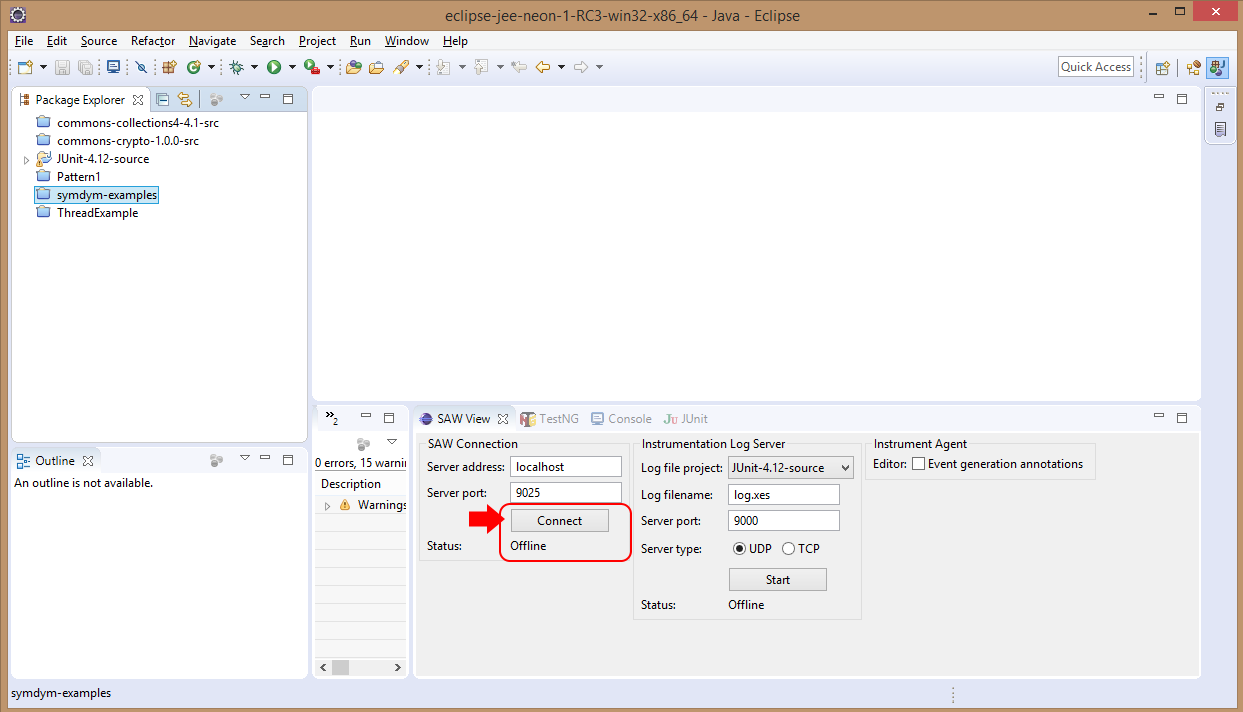
\includegraphics[width=0.8\textwidth]{gfx/eclipse-connect.png}
\caption{Connected the SAW Eclipse plugin after a model was discovered.}
\label{fig:connect}
\end{figure}

\subsubsection{Left panel: Activity overview and selection}
The panel on the left shows all the activities.
The search bar at the top allows one to lookup specific activites: it filters the list.
By selecting activities (left click), the corresponding parts in the center model will be outlined in red.
To select multiple activites, use control click.
To deselect, control click on selected activities.

In the case of hierarchical models, one can expand and collaps a subprocess / hierarchy 
level by clicking on the tree icons left of the activity names.
The activity list on the left and model in the center are linked:
expanding or collapsing in one view, will update the other.

\subsubsection{Right panel: Settings}
The right panel shows all the options to manipulate the discovery settings and analysis overlays.

The three big sliders on top manipulate the acitivty, path, and level depth filters for discovery.
The activities slider controls the fraction of activities that is included in log.
The paths slider controls the amount of noise filtering applied.
The level depth slider controls the amount of hierarchy levels shown / collapsed in the model.
When exploring hierarchical models, the level depth slider allows for a coarse grained exploration, 
while the plus and minus signs on the model allow for a fine grained exploration of the hierarchy.

Below the sliders are several setting buttons.
These buttons show the current settings for discovery and analysis.
When you click on these buttons, a popout allows you to set detailed settings.
There are four such settings buttons:

\paragraph{Discovery settings}
Setup the recursion and cancelation detection, as well as toggling basic tree rewrite simplification.

\paragraph{Visualization settings}
Choose the type of model shown, be it a statechart (Figure~\ref{fig:screen:vis:sc-vis}), 
sequence diagram, Petri net or process tree (Figure~\ref{fig:screen:vis:ptree-analysis}).
In addition, one can choose the model layout orientation.
For software logs, several activity label heuristics are availalble to reduce the activity names
without changing the discovered model (e.g., removing the package name from the labels).
Figure~\ref{fig:screen:vis:sc-vis} shows the Visualization settings panel.

\paragraph{Analysis settings}
Setup the metric overlays displayed on the model.
Different metrics can be calculated using either a fast approximation algorithm or the accurate alignment-based algorithms.
The following metrics are provided:
\begin{itemize}
    \item \textbf{Absolute Frequency} How often did the method call / activity occur?
    \item \textbf{Case Frequency} In how many traces did the method call / activity occur?
    \item \textbf{Log / Model Frequency} How many deviations from the discovered model are present in the log?
    \item \textbf{Error / Cancel Frequency} How many times a cancel / exception trigger occured?
    \item \textbf{Duration} What was the total duration of a method?
    \item \textbf{Own Duration} What was the duration of a method, minus the time spent in lower method calls?
    \item \textbf{Duration Efficiency} How much work was performed divided how much time? This can give an efficiency indication in case of multi-threaded code.
    \item \textbf{Resource Count} How many resources / threads were used to perform the method call / activity?
\end{itemize}
Figure~\ref{fig:screen:vis:ptree-analysis} shows the Analysis settings panel.

\paragraph{Export as}
Export the model and/or processed log either as an image, or as a ProM object for further analysis. 

\begin{figure*}[!ht]%
    \centering%
    \subfigure[
        Shown is the \emph{Statechart} model visualization with the \emph{Frequency metric} overlay. 
        In addition, the \emph{Visualization settings} panel is opened.
    ]{
        \label{fig:screen:vis:sc-vis}
        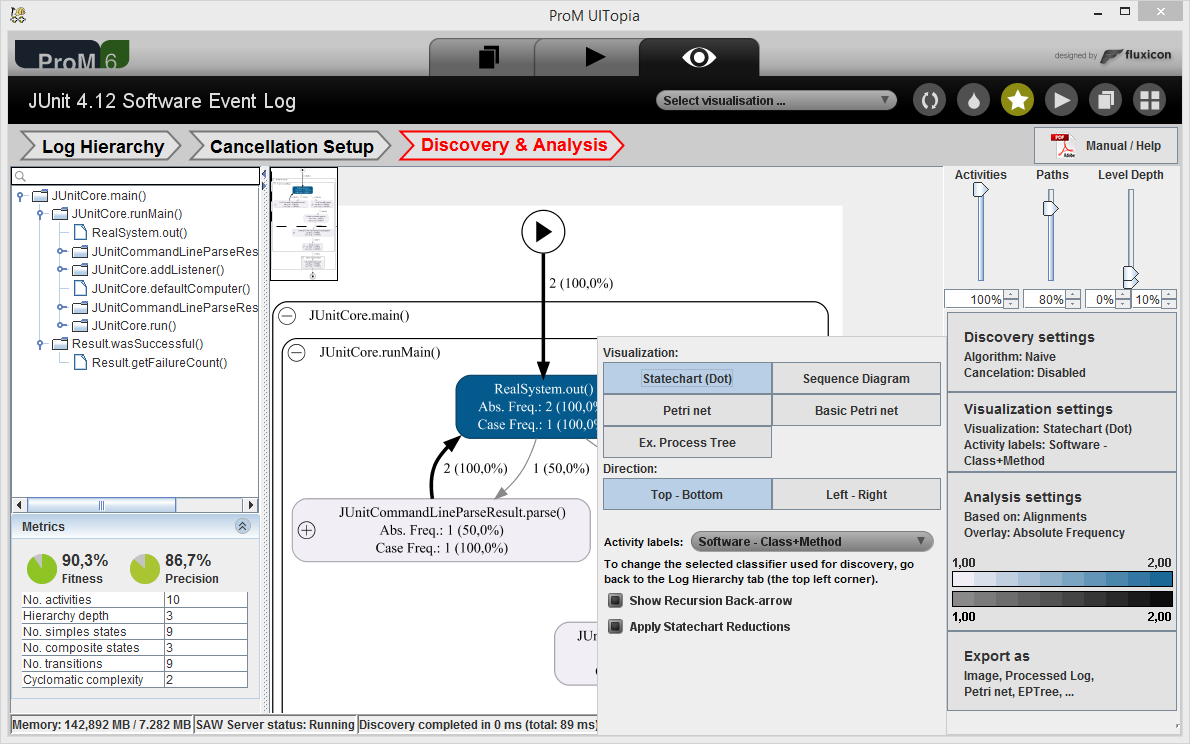
\includegraphics[width=0.94\textwidth]{gfx/model-sc-settings-vis.png}
    }
    \subfigure[
        Shown is the \emph{Process tree} model visualization with the \emph{Own Duration metric} overlay. 
        In addition, the \emph{Analysis settings} panel is opened.
    ]{
        \label{fig:screen:vis:ptree-analysis}
        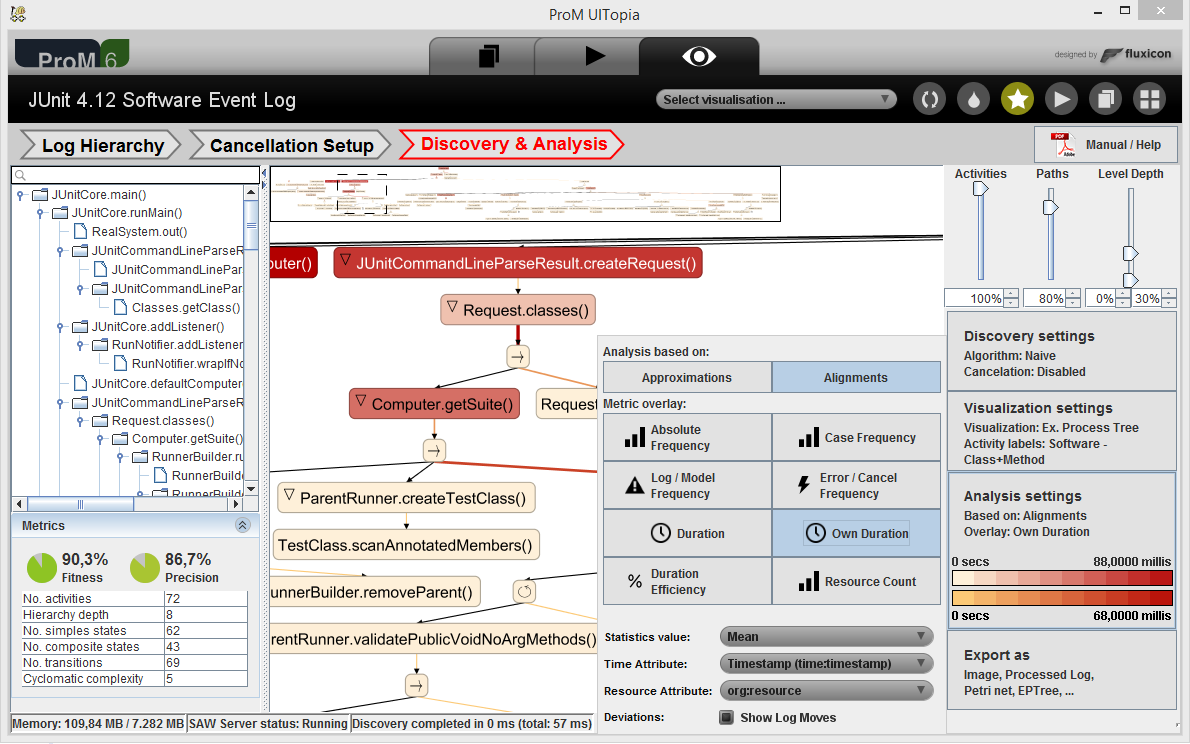
\includegraphics[width=0.94\textwidth]{gfx/model-ptree-settings-analysis.png}
    }
    \caption{The user interface after the tool
    discovered and annotated a model. 
    To the left, global metrics and a searchable alphabet summary is given. 
    In the middle, an interactive, zoomable model with mini-map is given.
    The model and alphabet views are linked. 
    To the right, the user can change various settings.}%
    \label{fig:screen:vis}%
\end{figure*}%

\end{document}
